\chapter{Suchalgorithmen}
\section{Systematische Suche}
Ein rationaler Agent sieht die Welt in verschiedenen Stati, z.B. wären da der aktuelle Zustand und der Zielzustand der Welt. Der rationale Agent muss jetzt eine Folge von Aktionen finden, welche ihn vom Initialzustand in den Zielzustand bringt.
\subsection{Voraussetzungen für eine Suche}
Ein rationaler Agent ist in den Ferien und muss so schnell wie möglich von Arad nach Bukarest , da dort sein Flieger geht. Wie schafft er das? Mit der Suche eines schnellstmöglichen Weges. \\ \newline
Generell kann man sagen, dass wenn die Umwelt folgende Eigenschaften erfüllt, der Agent eine \textbf{Sequenz von Aktionen} suchen kann, welche ihn zum Zielzustand führen werden:

\begin{enumerate}
	\item \textbf{Observable} - Der Agent weiss, wo er ist.
	\item \textbf{Static} - Die Umwelt verändert sich nicht plötzlich.
	\item \textbf{Deterministic} - Jede Aktion hat den gewünschten Effekt.
	\item \textbf{Discrete} - Nur eine finite Anzahl von Aktionen ist möglich in jedem Zustand.
\end{enumerate}

Im Beispiel Arad nach Bukarest sind diese Eigenschaften gegeben. Der Agent weiss, wo er sich befindet, die Städte verändern nicht plötzlich den Ort, und wenn er von einer Stadt in die nächste fährt, dann fährt er auch dorthin. Und, gegeben die Abstraktion, er kann nicht unendlich viele Städte direkt erreichen. Ein Status wäre hier z.B. die aktuelle Stadt auf der Karte, die Aktionen die Reise zwischen den Städten - also die Kanten des Graphen, die Aktionskosten die Distanz-Informationen auf den Kanten. 

\begin{figure}[h]
\centering
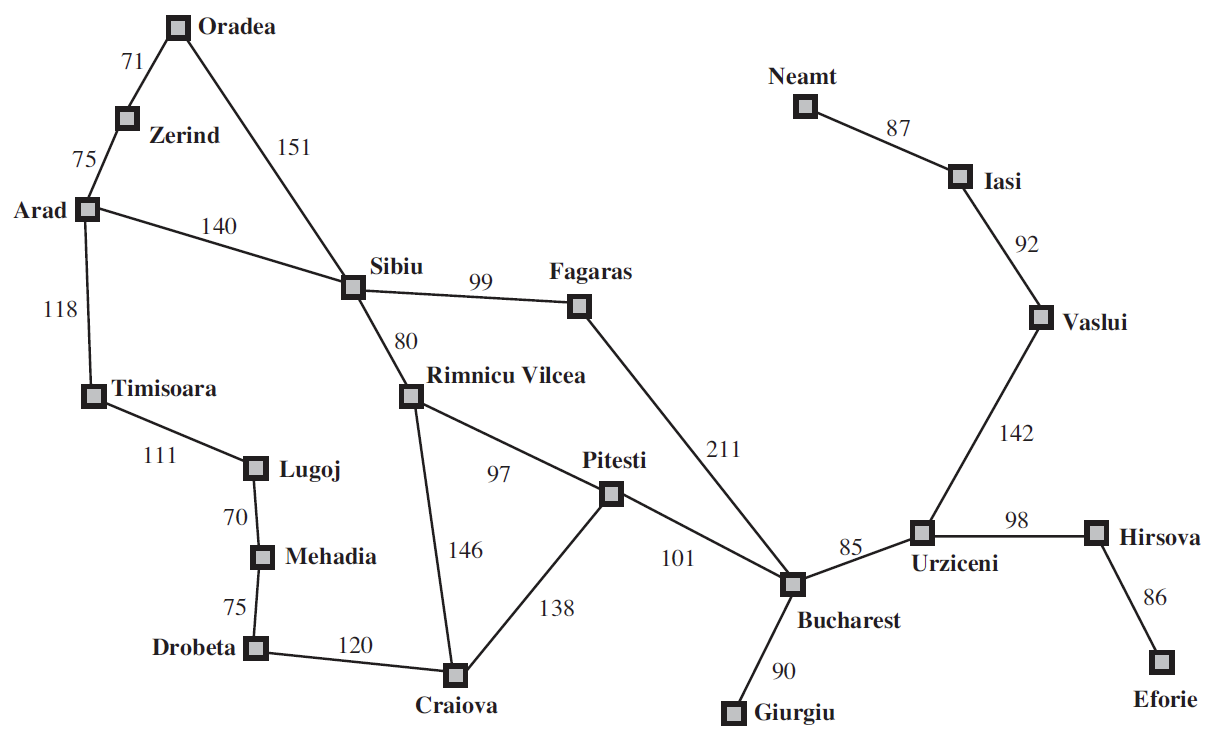
\includegraphics[width=0.5\linewidth]{fig/travel_example}
\caption{Beispiel für eine Umgebung wo eine Suche möglich ist}
\label{fig:travel_example}
\end{figure}

\subsection{Begrifflichkeiten}
\begin{description}
	\item[Initial State] Der erste Status des Agenten
	\item[State Space] Alle möglichen Stati (z.B. der Graph aller Städte)
	\item[Actions] Alle möglichen Aktionen
	\item[Transition Model] Eine Funktion, welche as Input einen Status und eine Aktion hat, und daraus einen neuen Status generiert. z.B. \texttt{succ(Arad, (Arad-Sibiu)) = Sibiu}.
	\item[Goal Test] Sind wir schon da? Sind wir schon da?
	\item[Path] Die Sequenz der Aktionen.
	\item[Path Costs] Die Kostenfunktion über den Gesamtpfad. Meistens die Summe der Kosten aller Einzelaktionen, aber z.B. bei einer Aktion 3 für 2 wäre es wieder anders.
	\item[Solution] Pfad vom Intialzustand zum Zielzustand.
	\item[Optimal Solution] Pfad vom Initialzustand zum Zielzustand mit den niedrigsten Kosten.
	\item[Search Costs] Die Kosten (Zeit \& Speicherverbrauch) um eine Lösung zu finden.
\end{description}

\subsection{Beispielmodelle}
\subsubsection{8 Puzzle}
\begin{figure}[h!]
\centering
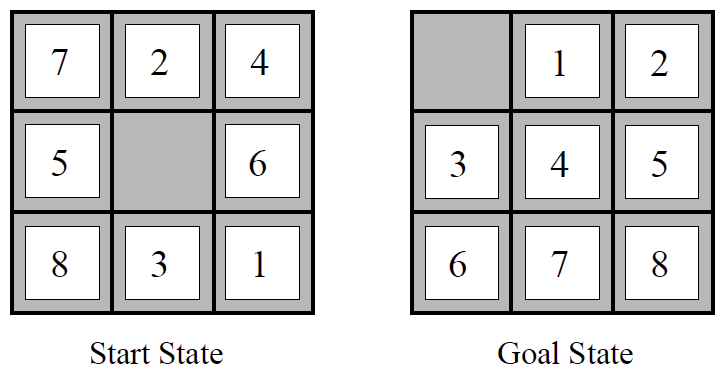
\includegraphics[width=0.6\linewidth]{fig/8_puzzle}
\caption{Das Spiel 8 Puzzle}
\label{fig:8_puzzle}
\end{figure}

In diesem Spiel wäre der aktuelle Status die Position der Spielsteine. Die Aktionen wären \textit{bewege das leere Feld} (simpler als die anderen zu bewegen) und der Goal Test wäre dann einfach \textit{ist der Zielzustand = aktueller Zustand}. Die Pfadkosten, sind hier definiert als jede Aktion kostet 1.

\subsubsection{8 Queens}
In diesem Spiel geht es darum, 8 Damen auf einem Feld so zu platzieren, dass keine Dame eine andere Dame bedroht. Hier ist der Zielzustand im Vorfeld unbekannt.
\begin{figure}[h!]
	\centering
	\begin{subfigure}[h]{0.2\textwidth}
	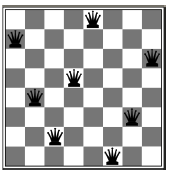
\includegraphics[width=\textwidth]{fig/8_queens_end}
		\caption{Zielzustand 1}
	\end{subfigure}
	~
	\begin{subfigure}[h]{0.2\textwidth}
	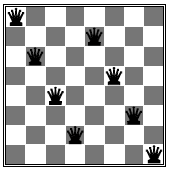
\includegraphics[width=\textwidth]{fig/8_queens_start}
		\caption{Zielzustand 2}
	\end{subfigure}
	\caption{Mögliche Zielzustände}
	\label{fig:send-receive-message}
\end{figure} 

Der aktuelle Status wäre wieder die Position der Damen auf dem Brett, der Initialstatus wäre ein leeres Brett, die \textit{Successor function}, dass man eine Dame zum Brett hinzufügt, und der Goal Test ist auch klar - es sind 8 Damen auf dem Brett die sich nicht bedrohen. Die Pfadkosten sind hier eigentlich egal, wir sind ja nur an der Lösung interessiert.

Optimaler wäre die Sucessor Function so zu definieren, dass man die Damen einfach Spaltenweise hinzufügt.

\subsection{Suchbäume}
\begin{figure}[h!]
	\centering
	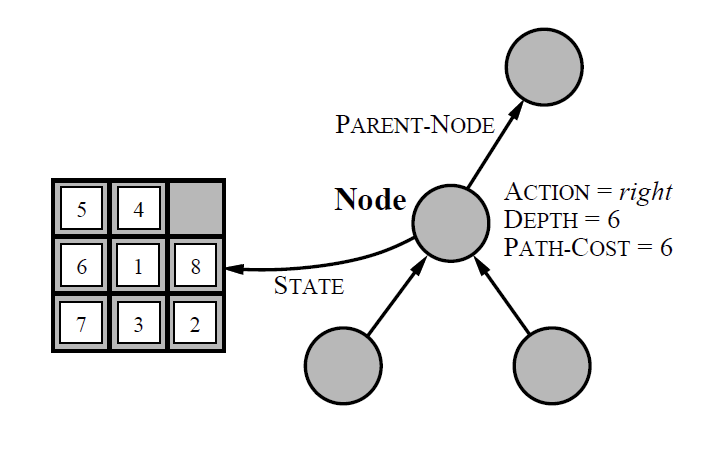
\includegraphics[width=0.5\linewidth]{fig/search_tree}
	\caption{Suchbaum Aufbau}
	\label{fig:search_tree}
\end{figure}
Ein Suchbaum beschreibt die Reihenfolge, in der Knoten im Suchraum besucht werden. Ein Knoten beschreibt dabei einen Status, die letzte Aktion, die zu ihm geführt hat (denn Status + Aktion = Status) und die aktuellen Pfadkosten. Er hat verschiedene Kinder, welche durch entsprechende Aktionen erreicht werden können.
\begin{description}
	\item[Frontier] Die Knoten, welche gerade von der Suchfunktion gefunden wurden und die noch nicht weiter untersucht werden.
	\item[Repeated State] Stati, welche im aktuellen Suchbaum schonmal vorkamen.
	\item[Redundant Paths] Wenn 2 Pfade gefunden werden, welche zum selben Status gelangen.
	\item[Search Space] = Suchraum. Ein Graph, indem die Knoten alle Stati im \textit{State Space} darstellen und die durch entsprechende Aktionen verbunden sind.
	\item [Node expansion] Generiert alle Nachfolge-Knoten, gegeben die Aktionen.
	\item []
\begin{figure} [h!]
\centering
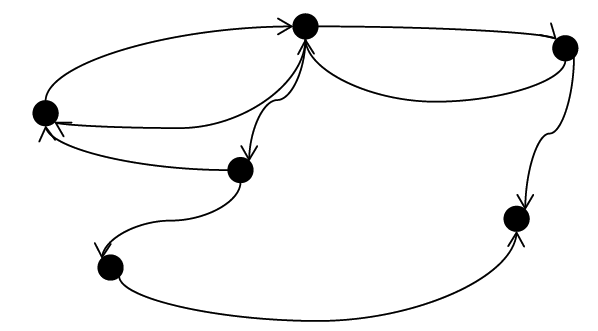
\includegraphics[width=0.2\linewidth]{fig/search_space}
\caption{Suchraum}
\label{fig:search_space}
\end{figure}
\end{description}


